\documentclass[11pt]{article}

\usepackage{fullpage}
\usepackage{amsmath}
\usepackage{amssymb}
\usepackage{amsthm}
\usepackage{fancyhdr}
\usepackage{algorithm}
\usepackage{algorithmic}
\usepackage{bm}
\usepackage{listings}
\usepackage{graphicx}
\usepackage{caption2}
\usepackage{subfigure}
\usepackage{float}
\usepackage{extpfeil}
\usepackage{color}
\usepackage[usenames,dvipsnames]{xcolor}


\newtheorem{theorem}{Theorem}[section]
\newtheorem{lemma}[theorem]{Lemma}
\newtheorem{corollary}[theorem]{Corollary}
\newtheorem{proposition}[theorem]{Proposition}
\newtheorem{definition}[theorem]{Definition}
\newtheorem{conjecture}[theorem]{Conjecture}
\newtheorem{remark}[subsection]{Remark}

%%
\newcommand\numberthis{\addtocounter{equation}{1}\tag{\theequation}}

%% define new symbols
\def\bx{\bm{x}}
\def\bb{\bm{b}}
\def\ba{\bm{a}}
\def\bc{\bm{c}}
\def\bf{\bm{f}}
\def\by{\bm{y}}
\def\bu{\bm{u}}
\def\bv{\bm{v}}
\def\BW{\bm{W}}
\def\BA{\bm{A}}
\def\bz{\bm{z}}
\def\BZ{\bm{Z}}
\def\BH{\bm{H}}
\def\BL{\bm{L}}
\def\BU{\bm{U}}
\def\BV{\bm{V}}
\def\BB{\bm{B}}
\def\BC{\bm{C}}
\def\BD{\bm{D}}
\def\BE{\bm{E}}
\def\BW{\bm{W}}
\def\BQ{\bm{Q}}
\def\BG{\bm{G}}
\def\BA{\bm{A}}
\def\BX{\bm{X}}
\def\BY{\bm{Y}}
\def\BQ{\bm{Q}}
\def\BI{\bm{I}}
\def\BR{\bm{R}}

%% define new brackets
\def\la{\left\langle}
\def\ra{\right\rangle}
\def\ln{\left\|}
\def\rn{\right\|}
\def\lb{\left(}
\def\rb{\right)}
\def\lsb{\left[}
\def\rsb{\right]}
\def\lcb{\left\{}
\def\rcb{\right\}}

%%
\DeclareMathOperator*{\argmin}{arg\,min}
\DeclareMathOperator*{\argmax}{arg\,max}

%%
\title{Homework I}
\author{Name: Shao Yanjun, Number: 19307110036}


\begin{document}
\maketitle
%------------------------------------
\begin{abstract}
This is Daniel's homework of  "Numerical Algorithms with Case Studies II".
\end{abstract}
%-------------------------------------
%=====================
\section{Problems}
\paragraph{Q1}
\subparagraph{(a)}
Notice that $\frac{\pi^2}{6}=\sum_{\mathbf{k}=1}^{\infty}\frac{1}{\mathbf{k}^2}$, we could claim that
\begin{align}
	|\frac{\pi^2}{6}-\mathbf{a}_n|&=|\sum_{k=n+1}^{\infty}\frac{1}{\mathbf{k}^2}|<
	|\sum_{k=n}^{\infty}\int_{k}^{k+1}\frac{1}{\mathbf{t}^2}\mathrm{d}\mathbf{t}|\\
	&=|\int_{n}^{\infty}\frac{1}{\mathbf{t}^2}\mathrm{d}\mathbf{t}|=\Theta(\frac{1}{\mathbf{n}})
\end{align}
\subparagraph{(b)}
The target value could be intepreted as $|\sum_{k=n+1}^{\infty}\frac{1}{\mathbf{k}^2}
-\frac{2}{2\mathbf{n}+1}|$, which suits the following inequality
\begin{align}
	|\sum_{k=n+1}^{\infty}\frac{1}{\mathbf{k}^2}
	-\frac{2}{2\mathbf{n}+1}| \le& 
	\min\{|\sum_{k=n}^{\infty}\int_{k}^{k+1}\frac{1}{\mathbf{t}^2}\mathrm{d}\mathbf{t}
		-\frac{2}{2n+1}|,
		|\sum_{k=n+1}^{\infty}\int_{k}^{k+1}\frac{1}{\mathbf{t}^2}\mathrm{d}\mathbf{t}
		-\frac{2}{2n+1}|\}\\
	&=\min\{|\int_{n}^{\infty}\frac{1}{\mathbf{t}^2}\mathrm{d}\mathbf{t}-\frac{2}{2n+1}|, |\int_{n+1}^{\infty}\frac{1}{\mathbf{t}^2}\mathrm{d}\mathbf{t}-\frac{2}{2n+1}|\}\\
	&= \frac{1}{(n+1)(2n+1)}=\Theta(\frac{1}{\mathbf{n}^2})	
\end{align}
\subparagraph{(c)}
Having recognize the decomposition of this series,
\begin{align}
	\sum_{k=1}^{\infty}\frac{1}{k(k+1)(k+2)}
	&=\sum_{k=1}^{\infty}(\frac{1}{2k(k+1)}-\frac{1}{2(k+1)(k+2)})\\
	&=\frac{1}{2}(\sum_{k=1}^{\infty}(\frac{1}{k}-\frac{1}{k+1})-\sum_{k=2}^{\infty}(\frac{1}{k}-\frac{1}{k+1}))=\frac{1}{4}
\end{align}
Therefore, the improvement can be furthered by the following formula, whose truncate remainder is reduced to $\Theta(n^{-3})$
\begin{align}
	\sum_{k=1}^{\infty}\frac{1}{k^2}&=1+\sum_{k=1}^{\infty}\frac{1}{k^2(k+1)}\\&=1+\sum_{k=1}^{\infty}\frac{2}{k^2(k+1)(k+2)}+\sum_{k=1}^{\infty}\frac{1}{k(k+1)(k+2)}\\
	&=\sum_{k=1}^{\infty}\frac{2}{k^2(k+1)(k+2)}+\frac{5}{4}
\end{align}
\paragraph{Q2}
The packs are uploaded with this pdf along with the semilogy plot. And for the difference in accuracy, I personally believe that with the larger scale of x in each iteration, the fluctuation from the actual value to the calculated value was enlarged at the same time. This was later reflected in the final converged result as a huge disturbence. Meanwhile, shifting all the value of x into the range of $(-\frac{\pi}{2}, \frac{\pi}{2}]$ is a wise improvement, because the impact of the  machine error is reduced.
\begin{figure}[H]
	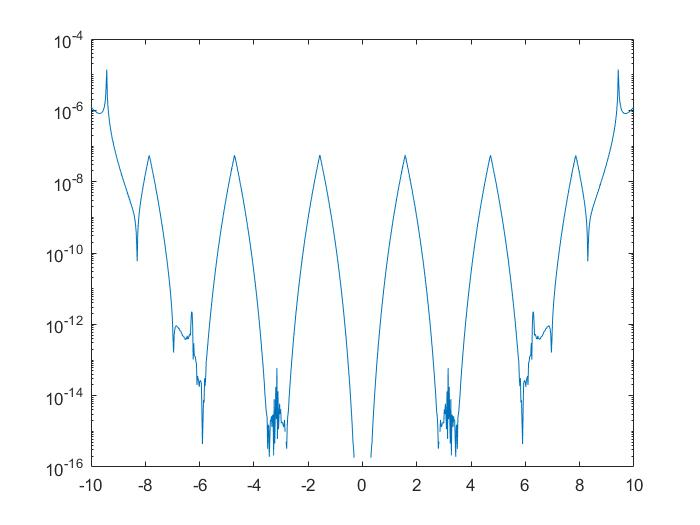
\includegraphics[width=0.6\linewidth]{H1Q2.jpg}
	\centering
	\caption{error}
\end{figure}
In this semilogy plot, we automatically regard the result of function sin\_with\_shift(x) as the true value of sin(x). It's not hard to observe that as the x starts to stay far away from zero, the calculated value also starts to stay inaccurate.
\paragraph{Q3}
Easy to notice that $\mathbf{b}=\mathbf{A}\mathbf{x_*}$, which suggests we look for two vector norms $\alpha$ and $\beta$ that satisfies $\|\mathbf{A}(\mathbf{x_*}-\mathbf{\hat{x}})\|_\alpha =  \|\mathbf{x_*}-\mathbf{\hat{x}}\|_\beta$. Therefore, we take $\alpha$ as norm(2) and define norm(A) for $\beta$ as follows,
\begin{align}
	\|\mathbf{x}\|_A = \sqrt{\mathbf{x^TAx}}
\end{align}
In this way, $\|\mathbf{b}-\mathbf{A\hat{x}}\|_2 =  \|\mathbf{x_*}-\mathbf{\hat{x}}\|_A$.
%-------------------------------------
%=====================
\end{document}
